\documentclass[12pt,a4paper]{amsart}
\usepackage{amsfonts}
\usepackage{amsthm}
\usepackage{listings}
\usepackage{amsmath}
\usepackage{amscd}
\usepackage[latin2]{inputenc}
\usepackage{t1enc}
\usepackage[mathscr]{eucal}
\usepackage{indentfirst}
\usepackage{graphicx}
\usepackage{graphics}
\usepackage{pict2e}
\usepackage{epic}
\numberwithin{equation}{section}
\usepackage[margin=2.9cm]{geometry}
\usepackage{epstopdf} 
\usepackage{graphicx}
\usepackage{grffile}
\usepackage{fancyhdr}
\usepackage{listings}
\usepackage{bookmark}

\def\numset#1{{\\mathbb #1}}
\def\R{{\mathbb R}}
\def\Q{{\mathbb Q}}
\def\Z{{\mathbb Z}}
\def\C{{\mathbb C}}
\def\S{{\mathbb S}}
\def\N{{\mathbb N}}
\def\H{{\mathbb H}}
\def\F{{\mathbb F}}
\def\PP{\mathbb P}
\def\A{{\mathbb A}}
\def\p{\partial}
\def\O{\Omega}
\def\a{\alpha}
\def\b{\beta}
\def\g{\gamma}
\def\G{\Gamma}
\def\d{\delta}
\def\D{\Delta}
\def\e{\varepsilon}
\def\r{\rho}
\def\t{\tau}
\def\l{\lambda}
\def\L{\Lambda}
\def\k{\kappa}
\def\s{\sigma}
\def\th{\theta}
\def\o{\omega}
\def\z{\zeta}
\def\n{\nabla}
\def\T{{\mathcal T}}
\def\X{{\mathcal X}}
\def\area{\mathrm{area}}
\def\dist{\mathrm{\rm dist}}
\def\diag{\mathrm{diag}}
\def\spt{\mathrm{spt\,}}
\def\diam{\mathrm{diam\,}}
\def\dim{\mathrm{dim\,}}
\def\graph{\mathrm{graph\,}}
\def\interior{\mathrm{interior\,}}
\def\diag{\mathrm{diag\,}}
\def\Image{\mathrm{Image}\,}
\def\osc{\mathop{\text{\rm osc}}}
\def\id{\operatorname{id}}
\def\im{\operatorname{im}}
\def\ker{\operatorname{ker}}
\def\rank{\operatorname{rank}}
\def\dim{\operatorname{dim}}
\def\Re{\operatorname{Re}}
\def\Im{\operatorname{Im}}

\def\suff{\implies}
\def\notsuff{\centernot\suff}
\def\nec{\impliedby}
\def\notnec{\centernot\nec}

\def\ra{\rightarrow}
\def\rai{\rightarrow\infty}

\newenvironment{solution}{\par\color{blue}\textbf{Solution:}}{\qed\color{black}}
\newenvironment{Part}[1]{\par\color{blue}\textbf{Part #1: }}{\qed}
\newenvironment{lemma}[1]{\par\color{blue}\textbf{Lemma #1: }}{}
\newenvironment{lemmaproof}{\par\color{blue}\textbf{Proof: }}{\qed}
\newenvironment{corollary}{\par\color{blue}\textbf{Corollary: }}


\theoremstyle{plain}
\newtheorem{Th}{Theorem}
\newtheorem{Lemma}[Th]{Lemma}
\newtheorem{Cor}[Th]{Corollary}
\newtheorem{Prop}[Th]{Proposition}

 \theoremstyle{definition}
\newtheorem{Def}[Th]{Definition}
\newtheorem{Conj}[Th]{Conjecture}
\newtheorem{Rem}[Th]{Remark}
\newtheorem{?}[Th]{Problem}
\newtheorem{Ex}{Example}

\newcommand{\Hom}{{\rm{Hom}}}
\newcommand{\ovl}{\overline}
%\newcommand{\M}{\mathbb{M}}

\pagestyle{fancy}
\renewcommand\headrulewidth{0pt}
\lhead{}\chead{}\rhead{}
\cfoot{\vspace*{1.5\baselineskip}\thepage}

\begin{document}

\title{Applications of Persistent Homology to Identifying Clusters in Graphs }


\author[]{M. Skilleter}

\address{Australian National University \\ Mathematical Sciences Institute} 


\begin{abstract} We study practical applications of persistent homology to identifying bridges in graphs. These graphs arise when analysing social networks, where bridges represent users who are members of multiple communities. In this paper, we outline several variations on an algorithm that utilises persistent homology and a metric on persistence diagrams, called the Wasserstein Distance, to identify cluster points. We also provide a mathematical justification for the efficacy of this algorithm and discuss ways in which it can be optimised to be applied to large data sets.
\end{abstract}

\maketitle

\section*{Introduction} The effect that a group of dedicated diffusers of malicious information can have is just beginning to be recognised. Private and state agencies are using platforms such as Twitter and Facebook to push their ideas, and the problem of identifying these information distributors is becoming more important. In this paper, we will demonstrate how techniques from the area of topological data analysis can be used to address this problem. Specifically, we will use ideas from persistent homology to identify bridges in graphs.

The field of topological data analysis (TDA) has been rising in prominence since the start of the 21st century. It utilises ideas from an area of mathematics called algebraic topology to draw inferences about large data sets by studying their structure when considered as a geometric object. 

As TDA becomes more widespread, various programming languages have added support. A full implementation of our algorithm in the language Julia can be found in our public GitHub repository \small{\textbf{https://github.com/OuroborosOfLife/Zigzag-Persistent-Homology/blob/master/Code/classifyingBridges.jl}}, making use of the package Eirene.

\section*{Definitions and Underlying Theory}

We begin by giving the relevant definitions, as well as stating some important theorems without proof.

\subsection*{Graph Theory}

A graph is a tuple $(V, E, \mu)$ with $V$ a set of vertices, $E$ a set of edges and $\mu : V \cup E \to \mathbb{R}_{\geq 0} \cup \{\infty\}$ a weight function. An edge between vertices $v_0$ and $v_1$ will be denoted by $(v_0, v_1)$. We call a graph \textit{undirected} if $(v_0, v_1) = (v_1, v_0)$ for every edge. All the graphs considered in this paper will be undirected and will have finite vertex and edge sets.

An important example of a weight function is the \textit{shortest path} weight function, which can be computed using Djikstra's Algorithm. Fix a vertex $v$ and for any other vertex $w$, define $\mu_v(w)$ to be the length of the shortest path from $w$ to $v$. For an edge $(v_0, v_1)$, we define $\mu_v((v_0, v_1)) = \max\{\mu_v(v_0), \mu_v(v_1)\}$.

The \textit{path-component} of a vertex $v$ is the subgraph of all vertices that can be reached from $v$. We call a graph \textit{connected} if it only has one path-component. Notice that if $v$ and $w$ are in different path components then the distance between them under the shortest path weight function is $\infty$.

\subsection*{Homology}

We will only define homology in the case of a graph, but these definitions can be generalised to any topological space. For a completely general definition of homology and for proofs of relevant theorems, see \cite{hatcher}.

For a graph $X = (V, E, \mu)$, we define two groups $C_0(X)$ and $C_1(X)$ by
\begin{align*}
C_0(X) &= \Z\{V\}  \\
C_1(X) &= \Z\{E\}
\end{align*}

For a set $S$, the notation $\Z\{S\}$ means that we take finite formal sums of elements in $S$ with coefficients in $\Z$. For example, if $S=\{s_0, s_1, s_2\}$ then $5s_0 - s_1 + 2s_2$ is an element of $\Z\{S\}$.  Elements of $C_0(X)$ are called $0$-chains and elements of $C_1(X)$ are $1$-chains.

We next define the boundary operator $d_1 : C_1(X) \to C_0(X)$. For an edge $e=(v_0,v_1)$, we set $d_1(e) = v_1-v_0$ (considered as a formal sum in $C_0(X)$). For an arbitrary $1$-chain, we now define
\[ d_1\left( \sum_i c_i e_i \right) = c_i \sum_i d_1(e_i) \]

Observe that we have defined $d_1$ on the basis $E$ and extended it linearly to arbitrary $1$-chains, so $d_1$ is a group homomorphism. Thus $\ker(d_1)$ and $\im(d_1)$ are subgroups. The homology groups $H_0(X)$ and $H_1(X)$ are then defined as
\begin{align*}
H_0(X) &= C_0(X) / \im(d_1) \\
H_1(X) &= \ker(d_1)
\end{align*}

Intuitively, one can think of $H_n(X)$ as measuring the number of $n$-dimensional ``holes'' in $X$. This idea is illustrated by the following example.

\begin{Ex} 
The circle $S^1$ can be thought of as a graph with a single vertex $v$ and a single edge $e = (v,v)$ which is a loop from $v$ to itself. To compute $d_1$, we evaluate it on the basis element $e$ to see that $d_1(e) = v-v = 0$. Thus $d_1$ is the zero map, so $\ker(d_1) = C_1(S^1) = \Z$ and $\im(d_1) = 0$. Therefore $H_0(S^1) = H_1(S^1) = \Z$. The single power of $\Z$ in $H_1(S^1)$ indicates that there is only one 1-dimensional ``hole'' in the circle which is exactly what one would expect. As we will see in the next theorem, the single $\Z$ in $H_0(X)$ shows that $S^1$ is connected.
\end{Ex}

A 0-dimensional hole is a gap between vertices that cannot be traversed, so one would hope for a relationship between the number of path-components and $H_0(X)$. Such a relationship is given by the following theorem.

\begin{Th}
(Proposition 2.7 in \cite{hatcher}) 
Suppose $X$ is a graph with $m$ distinct path-components. Then $H_0(X) = \Z^m$.
\end{Th}

This gives us an easy method for computing $H_0(X)$ by simply counting path-components. There is one other relation, however, that will significantly simplify our calculations of homology.

The Euler characteristic $\chi$ is a well-known graph invariant defined as $\chi = |V| - |E|$. Using homology, it can be shown that:

\begin{Th}
(Theorem 2.44 in \cite{hatcher})
The Euler characteristic of a graph $X$ is also given by $\chi = \rank(H_0(X)) - \rank(H_1(X))$. Here $\rank$ is the function defined by $\rank(\Z^m) = m$.
\end{Th}

We already know how to compute $\rank(H_0(X))$: by Theorem 1, this is the number of path-components in $X$. Because $H_1(X)$ is the kernel of a group homomorphism between free abelian groups, it is always a free group so the rank fully determines $H_1(X)$. Equating the two above expressions for $\chi$ and rearranging shows that $\rank(H_1(X)) = m - |V| + |E|$ where $m$ is the number of path-components in $X$. Thus the above two theorems give us a linear time method for computing homology.

\subsection*{Persistent Homology}

Extending homology is persistent homology, which is based on the idea that more information can be obtained from a graph by studying how $H_0(X)$ and $H_1(X)$ vary over time. To define this rigorously, we make use of filtrations. A filtration of a graph $X$ is a finite nested sequence of subgraphs $X_0 \subseteq X_1 \subseteq X_2 \subseteq ... \subseteq X$ which gives an inductive way to build $X$ one stage at a time.

Using the shortest path function $\mu_v$ defined earlier, we have a canonical way to obtain a filtration of $X$ associated to each vertex $v$. We set $X_0$ to be the point $v$, $X_1$ to be the subgraph of vertices distance $1$ away from $v$ and so forth. In general, $X_d$ is the induced subgraph of vertices distance $d$ or less from $v$. Figure \ref{filtration} below shows an example filtration of this sort, with $v$ the blue vertex and the colour gradually increasing in intensity as we radiate outwards from $v$.

\begin{figure}[h]
	\centering
	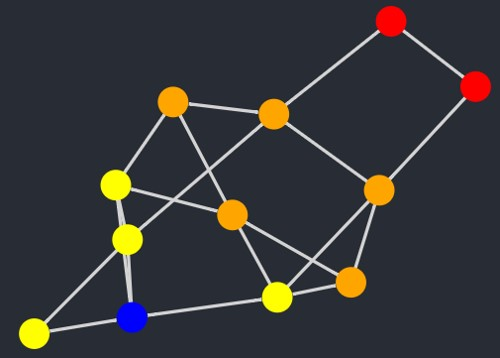
\includegraphics[scale=0.8]{ExampleFiltration.jpg}
	\caption{Example Filtration Using Shortest Path Function}
	\label{filtration}
\end{figure}

Once we have a filtration, we can build what are called the persistence diagrams. A persistence diagram is a multiset of pairs $(b,d) \in (\R \cup \{\infty\})^2$ representing the birth and death times of $n$-cycles (the elements of $H_n(X)$).  There is a persistence diagram associated with each dimension $n$. For example, because $H_0(X)$ measures path-components, the $0$-dimensional diagram tracks the births and deaths of path-components. This means that if two disjoint path-components become connected by a bridge at some stage in a filtration, one of the $0$-cycles will die at this stage. Because $H_1(X)$ measures $1$-dimensional holes, one can think of the $1$-dimensional persistence diagram as tracking the births and deaths of loops in $X$.

It is common to include the diagonal $\D = \{(r,r) : r \in \R\}$ in the persistence diagram so that any two persistence diagrams have the same cardinality. This allows us to find bijections between any two persistence diagrams, an important fact for the metric we will introduce shortly. In practise, however, all of our diagrams will be finite and of the same cardinality, so we will ignore this added layer of complexity. A persistence diagram without the diagonal is commonly called a persistence barcode and it is to these that we will refer for the rest of this paper.

One important feature which makes persistence barcodes so useful is that there is an associated metric, called the Wasserstein distance (in general this is only a pseudo-metric, but it will be a true metric for barcodes considered in this paper). The Wasserstein distance between two persistence barcodes $A$ and $B$ is given by
\[W_{p,q}(A,B)= \inf_{\substack{\eta: A \to B \\ \mbox{a bijection}}} \left(\sum_{a \in A} \| a-\eta(a)\|^p_q \right)^{1/p} \]

The values $p$ and $q$ are arbitrary positive integers (also possibly $\infty$). While different values of $p$ and $q$ can often reveal new information, for computational efficiency we will only use $p=q=2$.

In the particular case of our shortest path filtration, no 1-cycles will ever die and so $d=\infty$ for every pair in the 1-dimensional persistence barcode. This means that there is an explicit expression for the Wasserstein distance between two such 1-dimensional persistence barcodes \textit{so long as they have been sorted}. Since our algorithm generates sorted 1-dimensional persistence barcodes, we will make heavy use of this formula. 

Let $l$ denote the total number of 1-cycles in the graph $X$. We can represent 1-dimensional persistence barcodes as $l \times 2$ matrices where the $k^{th}$ row gives the birth and death times of the $k^{th}$ 1-cycle. Given two such persistence barcodes $\mathcal{B}^1$ and $\mathcal{B}^2$, their Wasserstein distance is
\[ W_{2,2}(\mathcal{B}^1, \mathcal{B}^2) = \sqrt{\sum_{k=1}^l |\mathcal{B}^1_{k, 1} - \mathcal{B}^2_{k,1} |^2} \]

This expression represents a marked increase in the efficiency of the algorithm. Computing the Wasserstein distance for arbitrary persistence barcodes involves solving an optimal matching problem (this is implemented in Julia using the Hungarian algorithm). The Hungarian algorithm has complexity $\mathcal{O}(l^3)$, so our $\mathcal{O}(l)$ formula scales far more effectively.


\subsection*{Bridges in Graphs}

The purpose of this paper is to develop an algorithm that identifies bridges in graphs, so we must make clear what is meant by a bridge. This is difficult to do rigorously (see \cite{bridgeDef}), but for intuition one should think of the following: a bridge between two clusters is a vertex which is connected to at least one vertex from each of the clusters.

It is important to emphasise that in our definition, a bridge is a vertex and not an edge as terminology sometimes varies across the computer science and sociology fields. We will not strictly adhere to the above definition of a bridge, but it is a useful starting point. As the reader sees example graphs, they will develop an understanding of what is meant by a bridge in a graph.

Conversely, a vertex which is not a bridge is called a cluster point and a collection of such cluster points is called a cluster. It is immediate that finding all bridges is equivalent to finding all cluster points and this will prove to be an easier problem.

Figure \ref{bridges} depicts six example graphs with bridges and cluster points distinguished by colour. Throughout this paper, unless specified otherwise, we will take the convention that red vertices are bridges and blue vertices are cluster points.

\begin{figure}[h]
	\centering
	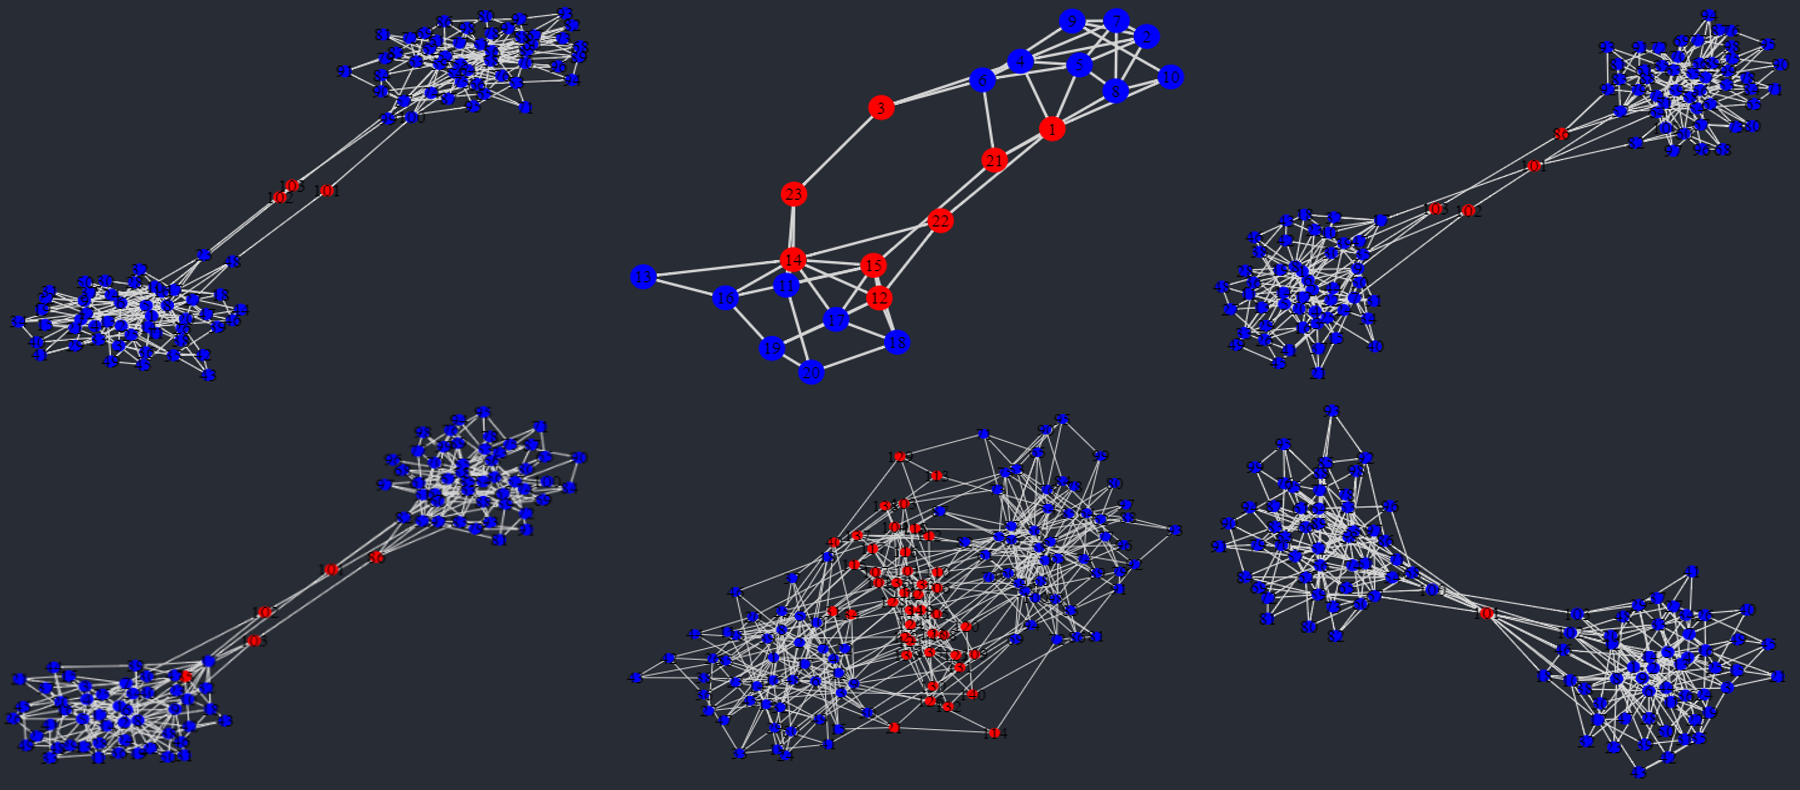
\includegraphics[scale=0.5]{BridgesDistinguished.jpg}
	\caption{Graphs with Bridges Distinguished}
	\label{bridges}
\end{figure}

\newpage

\section*{The Algorithm}

Here we will describe the development of our algorithm; for a summary, see the Discussion. For simplicity, we will first treat the case of graphs with two clusters and then consider how our algorithm can be generalised to graphs with arbitrary numbers of clusters. Before we describe the algorithm, however, we make the following observation. A vertex $v$ being a bridge is a local property in the sense that it only depends on the path-component of $v$. This means that we may assume without loss of generality that the graph $X$ is connected by simply running our algorithm on each path-component of $X$ separately. This is the first instance of parallelizability in the algorithm, since the existence of bridges in one path-component does not in any way affect bridges in other path-components. This assumption also allows us (by Theorems 1 and 2) to write $\rank(H_1(X)) = 1 - |V| + |E|$ which is how we calculate the 1-dimensional persistence barcodes for the shortest path filtration.

\subsection*{Early Attempts}

Continuing with this idea of locality, we describe our initial test for bridges which we shall call the ``neighbourhood test''. The underlying idea is that vertices far from $v$ should not affect whether or not $v$ is a bridge, so $v$ should be a bridge only if it is a bridge once we restrict to some small neighbourhood. Having restricted to a suitably small neighbourhood, we can now use more classical tests for bridges such as checking if removing $v$ disconnects the graph. As a first choice of small neighbourhood, consider the subgraph of vertices all directly adjacent to $v$. Figure \ref{nbhdTest} shows the neighbourhood test (with this choice of neighbourhood) applied to a typical graph.

\begin{figure}[h]
	\centering
	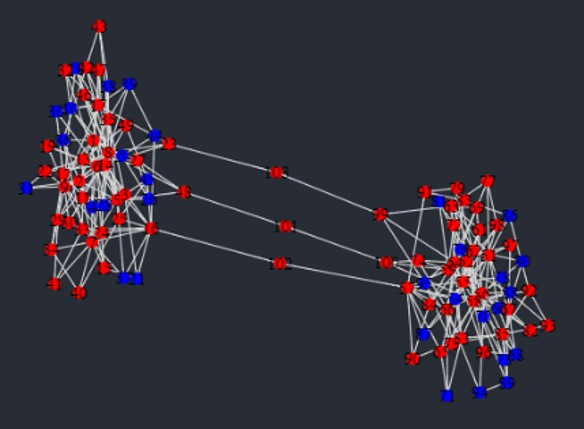
\includegraphics[scale=0.6]{NeighbourhoodTest.jpg}
	\caption{Neighbourhood Test Applied to Example Graph}
	\label{nbhdTest}
\end{figure}

While it is better to have false positives than to eliminate bridges, the neighbourhood test incorrectly identified a large number of cluster points as bridges. This problem can be resolved by taking a larger neighbourhood around each vertex, since removing $v$ from a larger neighbourhood is less likely to disconnect the graph. However, this method often eliminates parallel bridges such as those shown in Figure \ref{nbhdTest} because the parallel bridges are included in larger neighbourhoods, so removing $v$ no longer disconnects the subgraph.

One possible solution to this is to make the radius of the neighbourhood around each vertex dependent on $v$. This means that smaller radii can be chosen for parallel bridges to avoid the problem. However, there is no obvious way to choose a meaningful radius (doing so is almost identifying whether a vertex is a bridge or a cluster point). Instead, we introduce a generalisation of the neighbourhood test called the annulus test. 

\newpage

We define the closed annulus as $\D(v,a,b) = \{w \in V \mid a \leq \mu_v(w) \leq b\}$. Rather than choosing a radius dependent on $v$ for use in the neighbourhood test, we will check if $\D(v,a,b)$ is disconnected for sufficiently many $a$ and $b$. Since the neighbourhood test applied to the neighbourhood of radius $r$ about $v$ is simply checking if $\D(v,1,r)$ is disconnected, the annulus test is a true generalisation. Figure \ref{annulTest} shows the results of the annulus test applied to an example graph.

\begin{figure}[h]
	\centering
	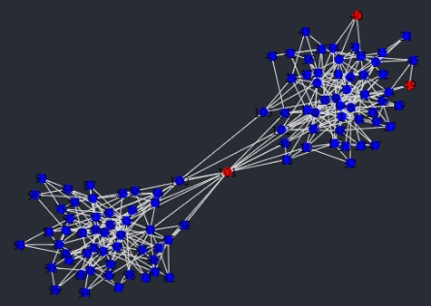
\includegraphics[scale=1]{AnnulusTest.jpg}
	\caption{Annulus Test Applied to Example Graph}
	\label{annulTest}
\end{figure}

While the annulus test was more accurate than the neighbourhood test across a range of graphs (compare Figures \ref{nbhdTest} and \ref{annulTest}), it still incorrectly identified some cluster points as bridges (such as those in the upper right of Figure \ref{annulTest}). This was surprising because, in general, the vertices which were classified incorrectly clearly belonged to clusters. To rectify this problem, the key observation was that the annulus test was not marking bridges as cluster points; it was only giving false positives. This meant that we could simply add further tests, now with the additional information of which nearby vertices were cluster points. 

By considering graphs such as Figure \ref{annulTest}, one might hope to find a meaningful way to say that two nearby vertices ``look similar'' so that if one has been identified as a cluster point then the other should be too. Persistent homology provides such a method by considering the persistence barcodes generated by the shortest path filtration. In a cluster, there are a large number of 1-cycles being born in quick succession because there is a high density of edges forming loops. For a bridge, though, there is an initial lull before a large number of births. Figure \ref{columnPlots} shows column plots for the number of 1-cycles born at each stage of the filtration. The left diagram corresponds to a typical cluster point and the right to a bridge.

\begin{figure}[h]
	\centering
	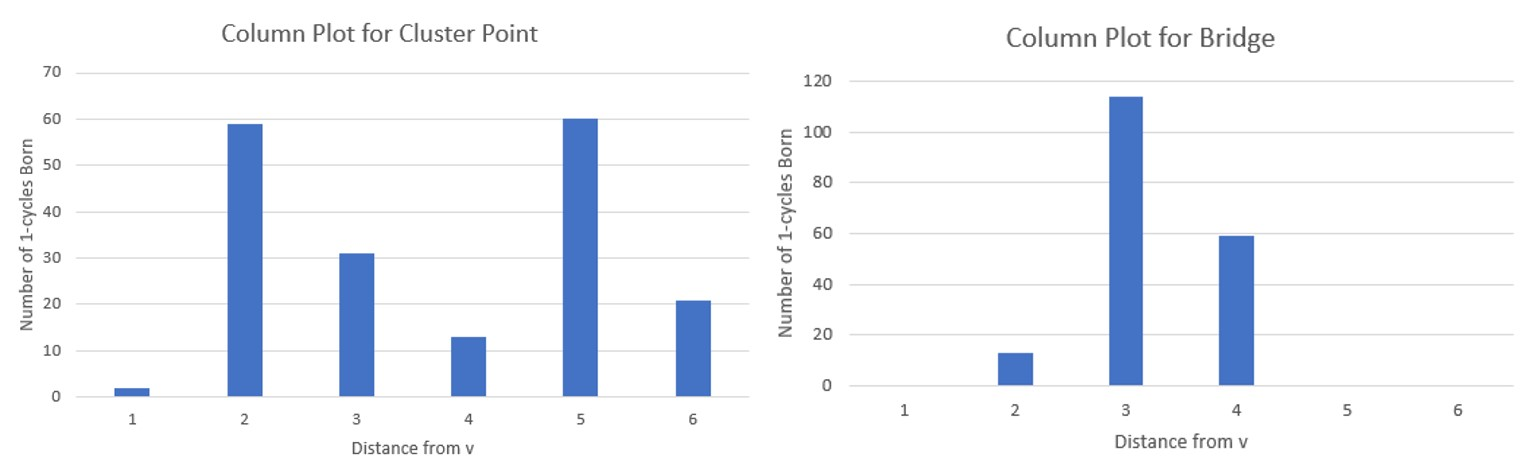
\includegraphics[scale=0.65]{ColumnPlots.jpg}
	\caption{Column Plots for Number of 1-cycles Born vs. Distance from $v$}
	\label{columnPlots}
\end{figure}

\newpage

The Wasserstein distance allows us to compare the $1$-dimensional persistence barcodes to find cluster points that may have been misidentified in our initial search for bridges. This is a significant simplification because it reduces our search to an extremal problem: we need only identify the vertices which are the most densely clustered and then use the Wasserstein distance to identify those neighbours which are also cluster points. 

There is one problem with this approach, which is that highly symmetric graphs can generate similar persistence barcodes for vertices which are quite far apart. There are cases where the persistence diagrams corresponding to vertices can be very close under the Wasserstein distance even though the vertices themselves are separated in the graph. In particular, there were instances of the algorithm identifying a bridge and a vertex lying at the edge of a sparse cluster. To address this, we only compare the persistence barcodes of vertices which are within a certain distance of one another.

\subsection*{Identifying Initial Cluster Points}

We now turn to the problem of finding vertices at the centres of clusters. The annulus test offers a partial solution but, in some cases, fails to identify any vertices if the cluster is sparsely connected (so that removing the inner circle disconnects the annulus for many values of $a$ and $b$). To motivate the following method, we return to the previous discussion about the times at which large numbers of 1-cycles are born. From Figure \ref{columnPlots}, one would expect the vertices at the centres of clusters to be those which have a large portion of the 1-cycles born early in the shortest path filtration. 

To identify the initial cluster points, we mark vertices for which a large number of births occur sufficiently early in the filtration. Currently, ``sufficiently early'' is taken to mean that the largest portion of 1-cycles is born less than some fraction $q$ of the way through the filtration. We want to take $q$ as small as possible because this test is not refined enough to distinguish between bridges and vertices on the edge of clusters. To do this, we start with the value $q=0.05$ and increment $q$ by $0.05$ until any initial cluster points are found. We then fix $q$ and stop searching for initial cluster points. 

\begin{figure}[h]
	\centering
	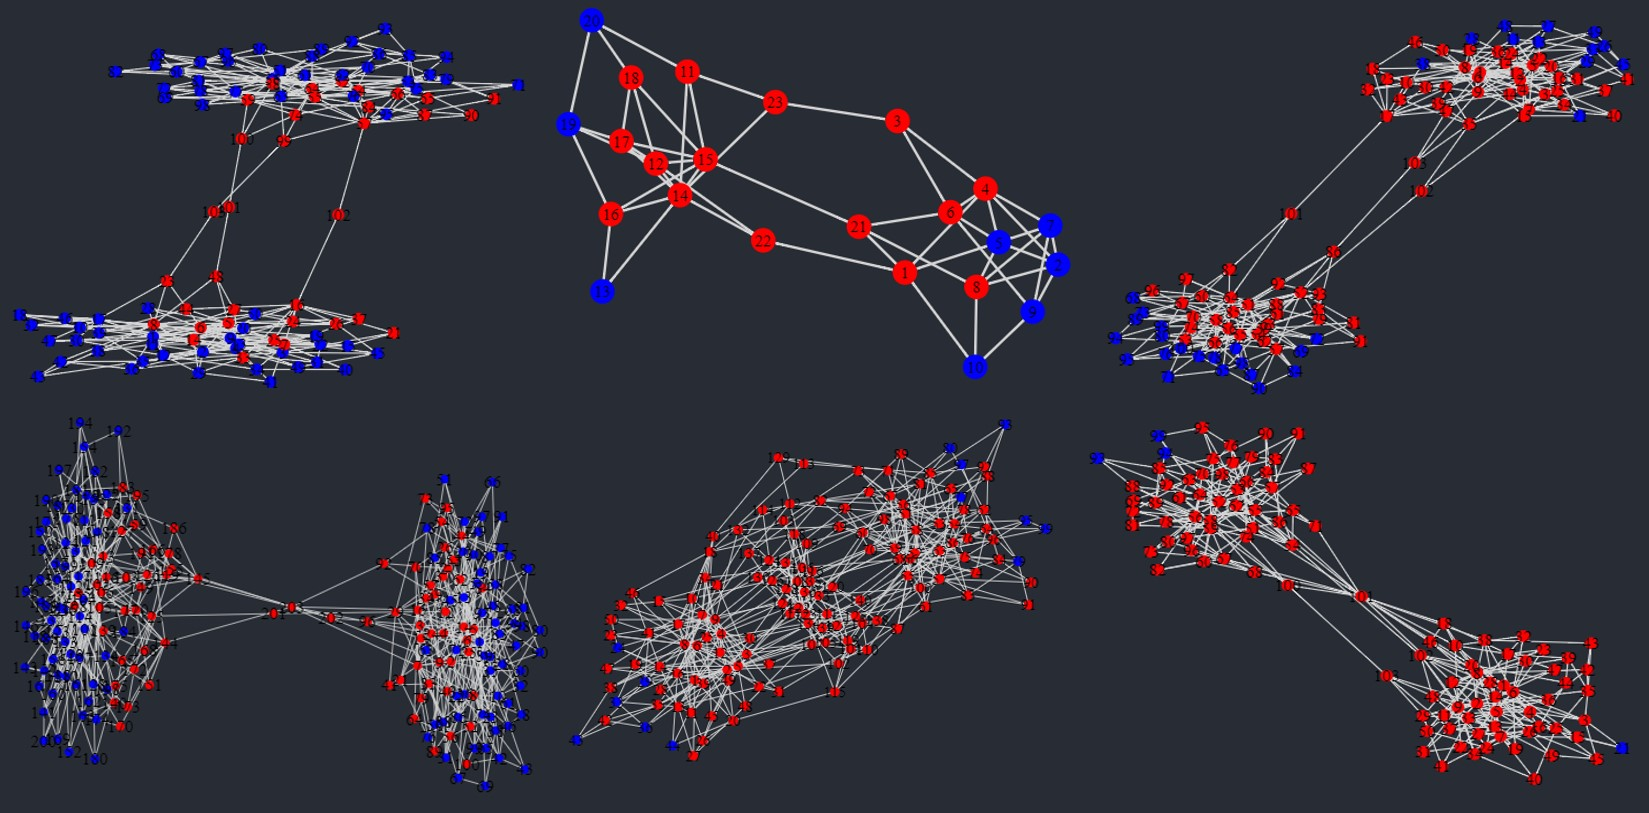
\includegraphics[scale=0.55]{InitialClusterPoints.jpg}
	\caption{Examples of Using 1-cycle Birth Times to Identify Cluster Points}
	\label{birthTimesTest}
\end{figure}

\newpage

Figure \ref{birthTimesTest} shows this method applied to various example graphs. In general, it will identify more vertices in densely connected clusters than in sparse clusters (compare the fourth and fifth graphs in Figure \ref{birthTimesTest}) simply because there are more 1-cycles in a densely connected cluster. The choice of $q$ discussed above gives us an easy solution to the extremal problem but it has some drawbacks that should be discussed: 
\begin{itemize}
	\item The fewer initial cluster points are identified, the more Wasserstein distance computations need to be made. If we are not using the shortest path filtration, calculating the Wasserstein distance is by far the most computationally expensive part of the algorithm.
	\item Suppose we have two distinct clusters, one densely connected and the other sparse. Because this test stops as soon as any cluster points have been identified, it is possible for cluster points in the dense cluster to be identified for small values of $q$ while no cluster points are identified in the sparse one. This means that we have no vertex to compare the rest of the sparse cluster against, so we could fail to identify an entire cluster.
\end{itemize}

Both of these issues can be resolved by using a larger value of $q$. However, there is no longer an obvious way to make $q$ dependent on the graph. This problem is still unresolved, but it is certainly an avenue for future research.

\subsection*{Graphs with More than Two Clusters}

We will now study how the algorithm performs on graphs with more than two clusters. Everything we have done thus far still holds in the general case and any assumptions (such as the connectedness of $X$) are still reasonable, for the same reasons as before.

The only real complication that arises with graphs with more than two clusters is that there are more opportunities for variation in the density of the clusters. This can cause the problem that, for a poor choice of $q$, we fail to identify any initial cluster points in some sparse cluster. We do not have a solution to this as of yet, so we will restrict ourselves to the class of graphs with clusters of similar densities. The majority of graphs used to model social networks fall into this class (see \cite{socialModels}) since communities tend to be densely connected.

As a partial solution should this problem occur, a user could manually identify some small set of initial cluster points and then proceed to use the Wasserstein distance to find the rest of the cluster.

Figure \ref{multiclusters} shows the results of applying the 1-cycle birth test, while Figure \ref{multiclustersfinal} shows the bridges and cluster points identified when the whole algorithm is applied to the same graphs. The accuracy of the algorithm is generally in keeping with the two cluster case.

\begin{figure}[h]
	\centering	
	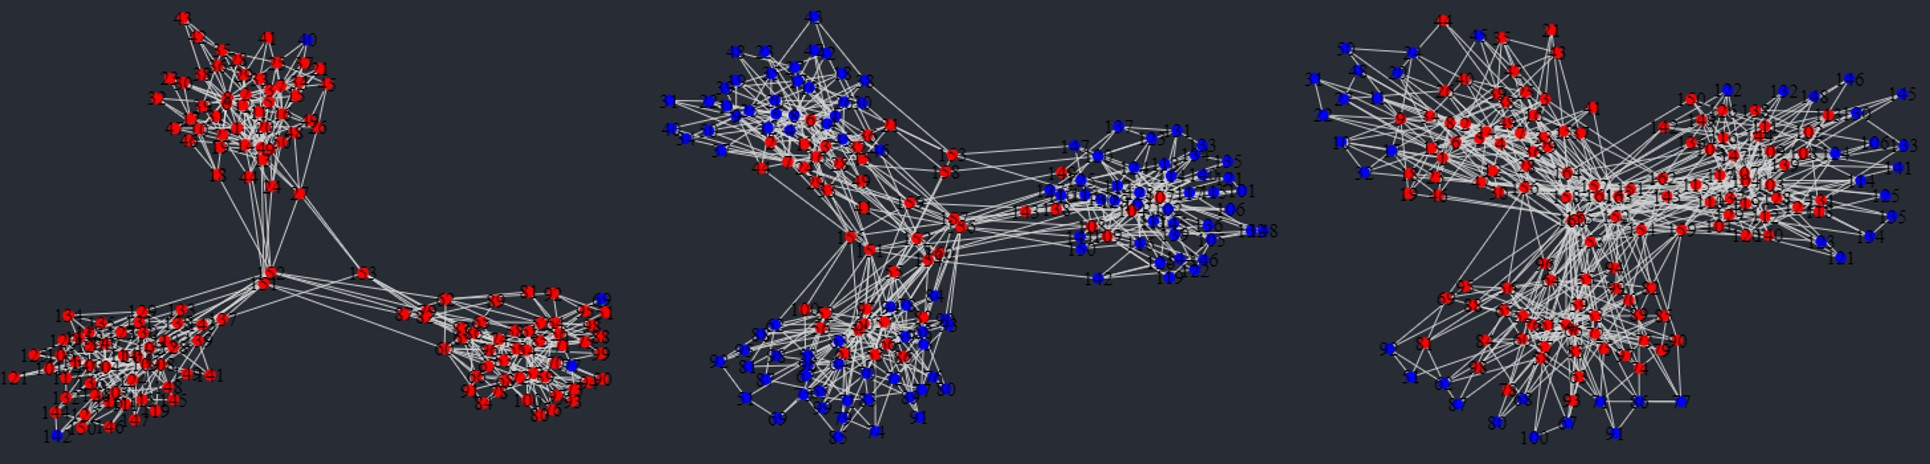
\includegraphics[scale=0.45]{Multiclusters.jpg}
	\caption{Initial Cluster Points Identified by 1-cycle Birth Test on Graphs with More Than Two Clusters}
	\label{multiclusters}
\end{figure}

\begin{figure}[h]
	\centering
	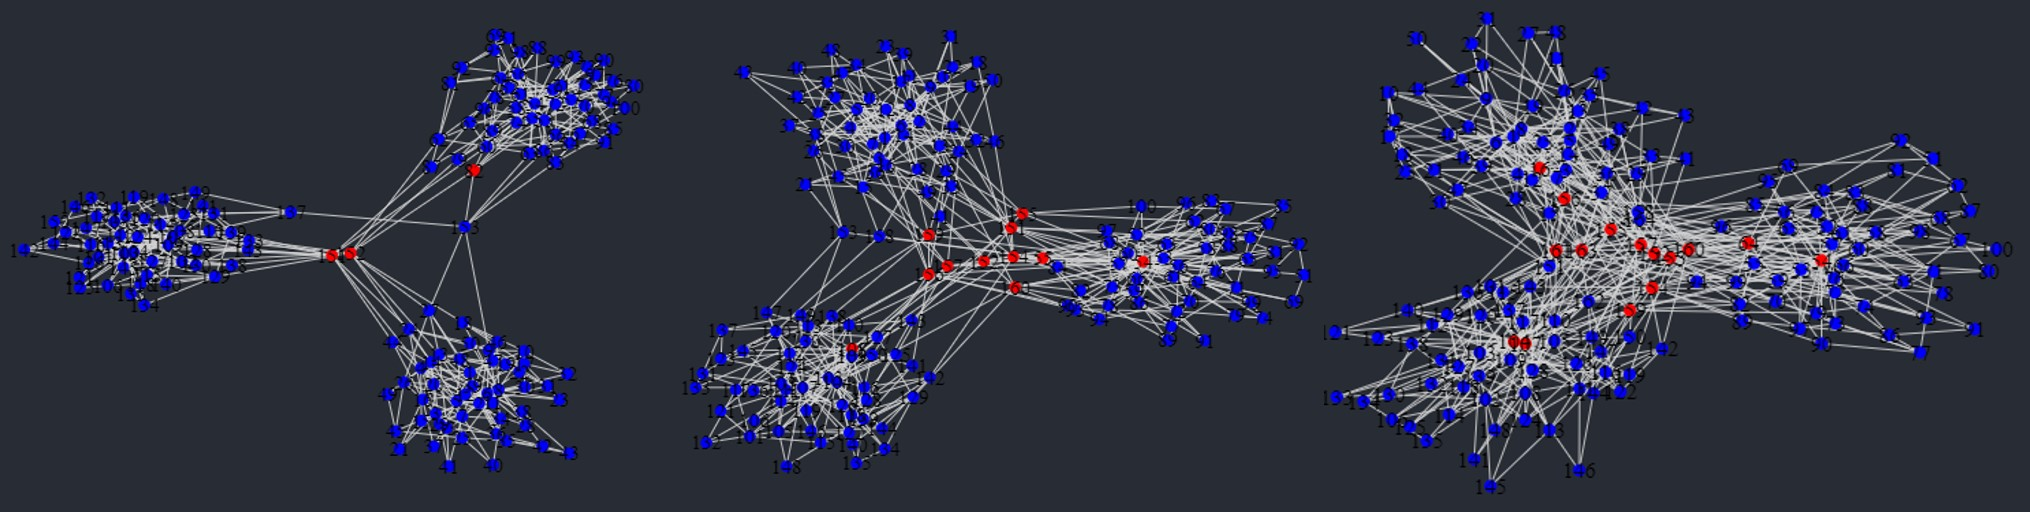
\includegraphics[scale=0.45]{MulticlustersFinal.jpg}
	\caption{Algorithm Applied to Graphs with More Than Two Clusters}
	\label{multiclustersfinal}
\end{figure}

If one does not wish to work with graphs with more than two clusters, it is theoretically possible to reduce to the two cluster case (we have not implemented this). Start by identifying a set of initial cluster points and designate some neighbourhoods of these points as being potential clusters. We then choose any two of these potential clusters (if there are $k$ potential clusters then there are $\binom{k}{2} = \frac{k(k-1)}{2}$ possible combinations) and include any vertices that lie between them as potential bridges. This gives rise to a connected subgraph which has at most two clusters, so we can run the algorithm from the two cluster case. We will not explore this approach as it would be more time-consuming than running the algorithm on the entire graph. Additionally, it still suffers from the problem of needing to identify initial cluster points to find the potential clusters.

\subsection*{Choosing the Upper Bound on Wasserstein Distance}

There is one final part of the algorithm that we should address, which is choosing the upper bound on the Wasserstein distance between persistence barcodes. Assume that we have identified a set of initial cluster points and now wish to compare their persistence barcodes against their neighbours' to identify the rest of the cluster. Given two vertices $v$ and $w$ with corresponding 1-dimensional persistence barcodes $A$ and $B$, we want to test if $W_{2,2}(A,B) \leq d$ for some upper bound $d$. As Figure \ref{upperBound} shows, the value of $d$ greatly affects the accuracy of the algorithm.

\begin{figure}[h]
	\centering
	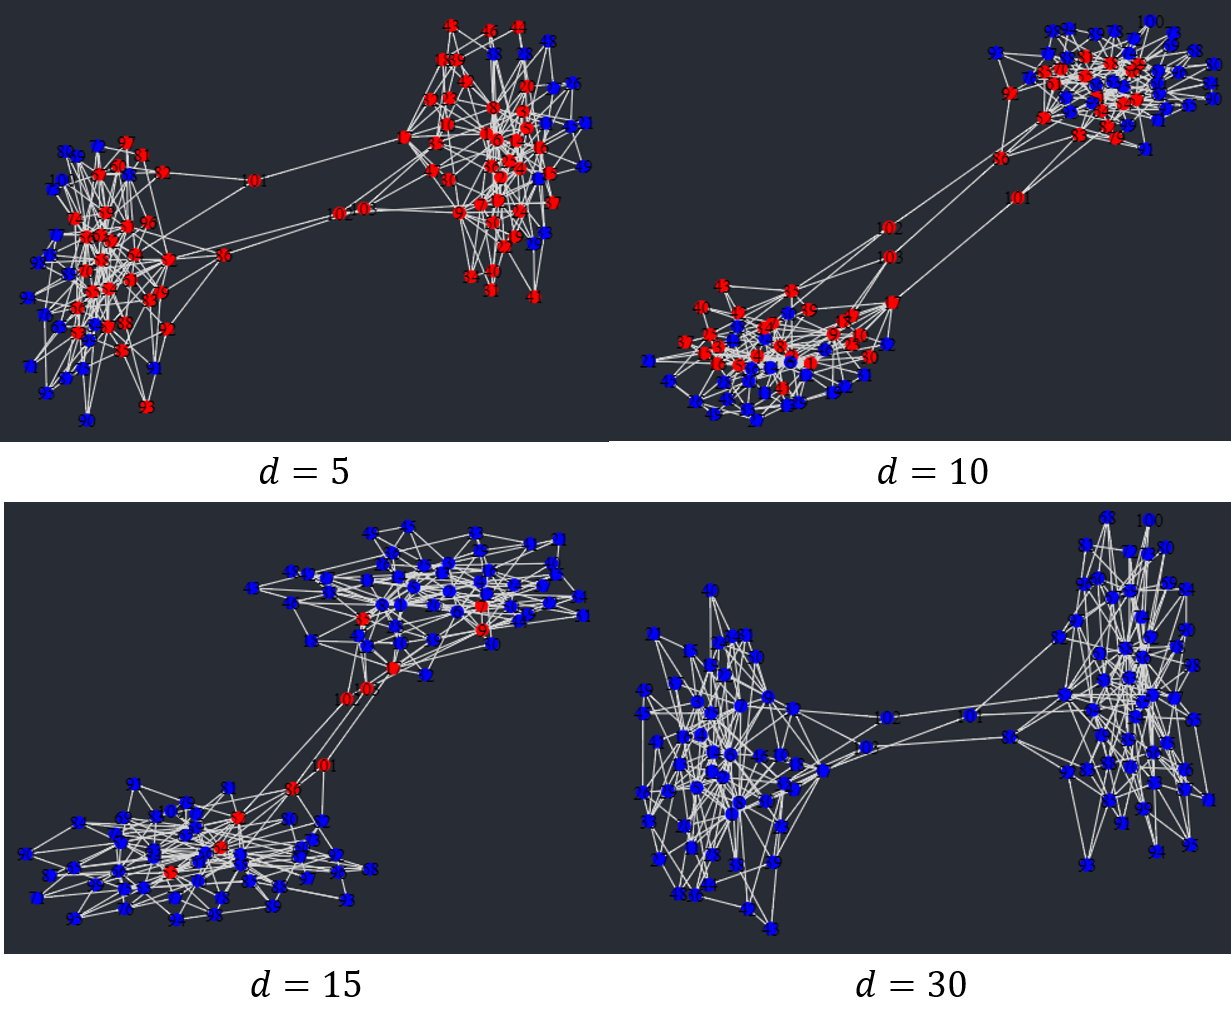
\includegraphics[scale=0.6]{UpperBound.jpg}
	\caption{Algorithm Applied to a Fixed Graph Using Different Values of $d$}
	\label{upperBound}
\end{figure}

\newpage

One can think of $d$ as the radius of the cluster under the Wasserstein distance. If we already knew the set $S$ of persistence barcodes corresponding to cluster points, we could use the standard definition of radius as $\frac{1}{2}\sup_{A,B \in S} W_{2,2}(A,B)$. Unfortunately, we are  trying to use the radius to identify $S$ so this isn't possible. Instead, we want a definition that doesn't depend on knowing $S$ but is as close as possible to the above value.

This can be accomplished as follows: suppose we have already identified a cluster point $c$ and a bridge $b$. The 1-dimensional persistence barcodes (call them $C$ and $B$ respectively) corresponding to these vertices should be the most separated in the graph. The value $W_{2,2,}(C,B)$ is, in some sense, the ``diameter'' of the graph under the Wasserstein distance because it is the largest possible Wasserstein distance between any two persistence diagrams. We thus define $d$ by
\[ d = \frac{1}{2} W_{2,2}(C,B). \]
In general, this is a good value of $d$. For example, Figure \ref{ideald} shows the same graph as in Figure \ref{upperBound} with $d=18.76$, the value given by this formula.

\begin{figure}[h]
	\centering
	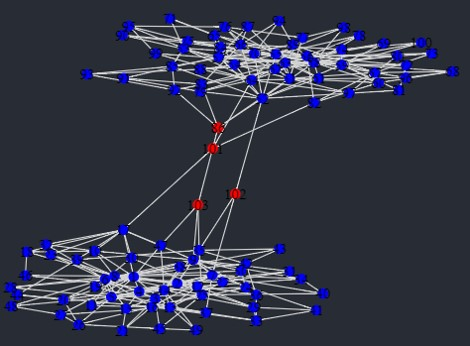
\includegraphics[scale=0.8]{IdealBridges.jpg}
	\caption{Graph with Value $d=18.76$ Chosen Using Diameter Method}
	\label{ideald}
\end{figure}
	
\newpage
	
The obvious drawback to this method is that it requires knowing a bridge beforehand. To avoid this problem, we can compute the Wasserstein distance between \textit{all} pairs of vertices and choose the maximum value to be the diameter. For a general filtration, this is quite computationally inefficient because of the expense of the generic algorithm for computing the Wasserstein distance. However, using our explicit formula for Wasserstein distance makes this approach feasible in the case of the shortest path filtration. 


\section*{Discussion}

We will now discuss the accuracy of the algorithm, as well as some potential avenues for further research. The algorithm is summarised here, along with estimates on the complexity of each stage:
\begin{enumerate}
	\item Compute the shortest path distance between all pairs of vertices using Djikstra's algorithm. This is known to be complexity $\mathcal{O}(|E|+|V|\log |V|)$.
	\item Using the Euler characteristic formula for rank of the first homology, compute the 1-dimensional persistence barcodes associated with each vertex. For each vertex, we must check which vertices and edges are included at each stage of the shortest path filtration. Thus the total complexity is $\mathcal{O}(|V|(|V|+|E|))$ 
	\item Identify initial cluster points by looking for vertices for which a large number of 1-cycles are born early in the shortest path filtration. Having already computed the 1-dimensional persistence barcodes, this is $\mathcal{O}(|V|)$.
	\item Compute the Wasserstein distance between the 1-dimensional persistence barcodes associated to all pairs of vertices. Since the length of each such barcode is $1-|V|+|E|$, this is complexity $\mathcal{O}(|V|^2(|E|-|V|))$.
	\item Using the results of the previous stage, compute $d$ as half the maximum Wasserstein distance and identify all vertices which are within $d$ of the initial cluster points. Any unidentified vertices are the bridges. This only involves using stage (4) to identify which pairs of vertices are within $d$ of each other (under the Wasserstein distance) and so this stage is complexity $\mathcal{O}(|V|^2)$.
\end{enumerate}

Other clustering methods are of cubic complexity, so our algorithm is comparable in terms of efficiency (see \cite{spectral}).

\newpage

\subsection*{Comparison with a Classical Clustering Method} To justify the use of 1-cycle birth times to identify initial cluster points, we compare this test to a more classical method for clustering. We will assume that our graph has only two clusters because this method only allows us to \textit{bipartition} a graph. We define the Laplacian matrix $L$ for a graph by the formula
\[ L_{i,j} = \begin{cases} \deg(v_i) & \mbox{if $i=j$} \\ -1 & \mbox{if $v_i$ is adjacent to $v_j$} \\ 0 & \mbox{otherwise} \end{cases} \]

The matrix $L$ is symmetric and positive-semidefinite, so its eigenvalues are all real and non-negative. An easy result in spectral clustering (see \cite{fiedler}) is that the multiplicity of the eigenvalue $\l = 0$ is exactly the number of path-components in $X$. By our assumption that $X$ is connected, this means that $\l = 0$ always has multiplicity $1$.

The smallest non-zero eigenvalue of $L$ is called the spectral gap. By the above, the spectral gap will always be the second eigenvalue when they are ordered. The associated eigenvector is called the Fiedler vector and it gives us a method for partitioning $X$ into two connected clusters which we will now describe. Let $s$ denote the spectral gap and $f$ denote the Fiedler vector, so $Lf = sf$. Because eigenvectors are only defined up to scaling by a non-zero constant, we will have to check that any information we deduce from $f$ is invariant under scaling. 

For each vertex $v_i$, the sign of the $i^{th}$ entry of $f$ tells us which of the two clusters $v_i$ should belong to. That is, if the signs of $f_i$ and $f_j$ are different then $v_i$ and $v_j$ belong to different clusters. This property is clearly preserved under scaling because, although scaling by a negative constant value may change the sign of the entry, it will always preserve the property of having different signs.

Building on this, the magnitude of $f_i$ directly relates to how close to the centre of a cluster $v_i$ is. To account for scaling, we identify those vertices for which $|f_i|$ is greater than the mean as being initial cluster points. To show that this is invariant under scaling, suppose that $X$ has $n$ vertices and that $|f_i| > \frac{\sum_j |f_j|}{n}$. Then
\begin{align*}
|(cf)_i| &= |c| \cdot |f_i| \\
&> |c| \cdot \frac{\sum_j |f_j|}{n} \\
&= \frac{\sum_j|c| \cdot |f_j|}{n} \\
&= \frac{\sum_j |(cf)_j|}{n}
\end{align*}

Thus this property is well-defined under scaling. To determine if our test using 1-cycle birth times produces reasonable results, let us compare it to the vertices identified by the Fiedler vector. Figure \ref{fiedlerTest} shows the results of using the Fiedler vector applied to the same graphs as in Figure \ref{birthTimesTest}. 

\begin{figure}[h]
	\centering
	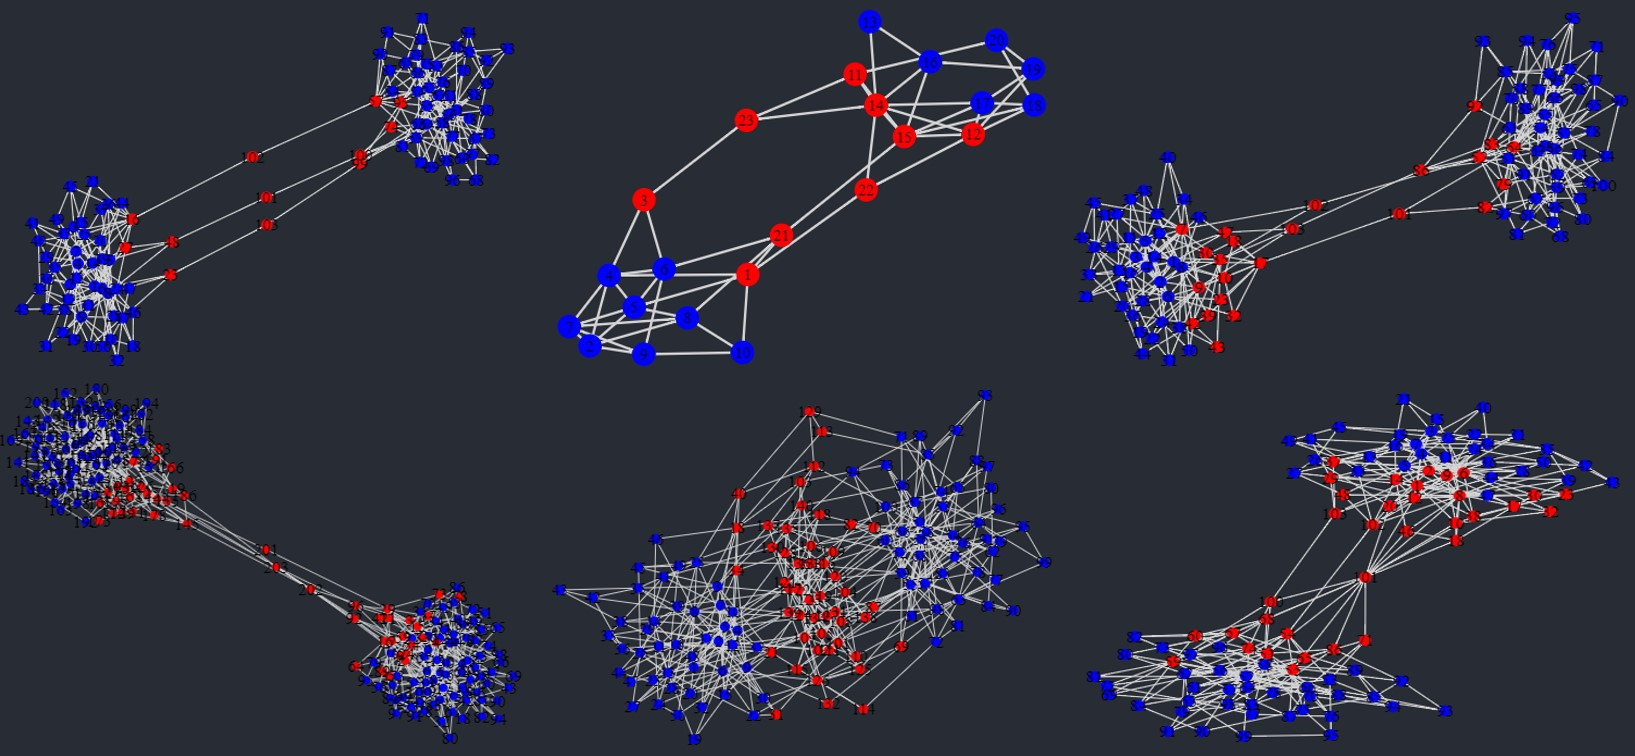
\includegraphics[scale=0.55]{FiedlerClusterPoints.jpg}
	\caption{Example of Using Fiedler Vector to Identify Cluster Points}
	\label{fiedlerTest}
\end{figure}

\newpage

In general, the Fiedler vector identifies as many or more initial cluster points, as illustrated by comparing Figures \ref{birthTimesTest} and \ref{fiedlerTest}. In fact, not once across twenty test graphs did the 1-cycle test identify a vertex as a cluster point that the Fiedler vector did not. Unfortunately, there is no generalisation of the Fiedler vector for graphs with more than two clusters. However, that the 1-cycle test and the Fiedler vector agree in the two cluster case supports the accuracy of our method. If one chooses to reduce to the two cluster case, the Fiedler vector offers an alternate method of identifying the initial cluster points.

\subsection*{Alternative Models for Social Networks} Much of this algorithm has been built around the use of the shortest path filtration. However, for use in identifying diffusers of information in social networks, there is at least one other filtration worth considering. This is called complex contagion, which relies on the idea that a frequently shared message will build momentum; it will "go viral". Using complex contagion to model a social network gives rise to a weighted directed graph, where the value of the edge $(v_0,v_1)$ is the probability of $v_0$ sending a message to $v_1$. 

For a given vertex $v$, we still have an associated filtration constructed in the same way as the shortest path filtration. The problem in using this filtration lies in the fact that the graph $X$ is directed: homology theory is developed in the language of topological spaces which have no concept of direction. Thus much of the underlying theory of persistent homology (such as the existence of the persistence barcode) is lost. We can rectify this by assuming that the probability of $a$ contacting $b$ is the same as $b$ contacting $a$, giving rise to a weighted, but undirected, graph that our algorithm can be applied to. The use of the complex contagion filtration is not one that we have tested, but it would certainly be worth considering in the future. 

There are also methods for building higher-dimensional models for social networks (see \cite{highdim}). Currently, the groups $H_0(X)$ and $H_1(X)$ are the only non-zero homology; in this paper, we defined them this way but it is actually a non-trivial result relying on the fact that $X$ is what is known as a cellular complex. A higher-dimensional model would allow for non-trivial higher homology groups, giving us more information about the geometric structure of $X$. The largest potential problem with this is that we could no longer use the Euler characteristic to compute homology. The formula for the Euler characteristic does generalise as an alternating sum of the ranks of homology groups, but we no longer have equally many equations as unknowns. There are other methods for computing persistence barcodes (one such is implemented in Julia via Eirene) but these tend to be of cubic complexity, as opposed to being linear time.  

Using a higher-dimensional model would allow us to make Wasserstein distance computations across multiple dimensions of persistence barcodes. The hope is that this would refine the ability to find other cluster points given an initial set, because a cluster could be considered as a higher-dimensional object while a bridge would generally just be 1-dimensional. However, we would not be able to use the explicit formula for the Wasserstein distance on higher-dimensional barcodes. In fact, if any 1-cycles die due to these higher-dimensional structures, this formula would no longer be valid even in the 1-dimensional case. The low complexity of our algorithm is extremely dependent on the shortest path filtration.

\subsection*{Conclusion}

In this paper, we have developed an algorithm which identifies bridges in graphs. This algorithm provides a method for identifying diffusers of malicious information over social media by modeling networks as graphs and identifying the bridges in these graphs as diffusers.

Our algorithm can alternatively be viewed as a method of clustering, another important problem. By partitioning the vertices of the graph into clusters and bridges, we solved the equivalent problem of identifying cluster points by considering the births of 1-cycles, leading naturally to the use of persistence barcodes and persistent homology in general. Comparison with an existing clustering method shows that our algorithm gives reasonable results and it is of a comparable complexity to existing methods of clustering. 

Overall, our algorithm provides a novel solution to the problem of identifying bridges in graphs which is both accurate and efficient.

\newpage

\begin{thebibliography}{99}

\bibitem{hatcher} A. Hatcher (2002). \textit{Algebraic Topology}. Cambridge University Press. Available at \textbf{https://pi.math.cornell.edu/~hatcher/AT/AT.pdf}.

\bibitem{geom} M. Kerber, D. Morozov, A. Nigmetov (2016). \textit{Geometry Helps to Compare Persistence Diagrams}. Available at \textbf{https://arxiv.org/abs/1606.03357}.

\bibitem{fiedler} B. Slininger. \textit{Fiedler's Theory of Spectral Graph Partitioning}. Available at \textbf{http://citeseerx.ist.psu.edu/viewdoc/download?doi=10.1.1.592.1730\&rep=rep1\&type=pdf}.

\bibitem{highdim} D. Spivak (2009). \textit{Higher-dimensional models of networks}. Available at \textbf{https://arxiv.org/abs/0909.4314}.

\bibitem{graphlinks} S. Bhatia, B. Chatterjee, D. Nathani, M. Kaul (2018). \textit{Understanding and Predicting Links in Graphs: A Persistent Homology Perspective}. Available at \textbf{https://arxiv.org/abs/1811.04049}.

\bibitem{spectral} D. Yan, L. Huang, M. Jordan. \textit{Fast Approximate Spectral Clustering}. Available at \textbf{https://people.eecs.berkeley.edu/~jordan/papers/yan-etal-long.pdf}.

\bibitem{bridgeDef} D. Centola, M. Macy. \textit{Complex contagions and the weakness of long ties}. In: American Journal of Sociology 113.3 (2007), pp. 702-734.

\bibitem{socialModels} R. Ram, M. Rizoiu (2019). \textit{A social science-grounded approach for quantifying online social influence}. In: Australian Social Network Analysis Conference (ASNAC'19) (p. 2). Adelaide, Australia.

\end{thebibliography}

\newpage

\section*{Code}

\begin{lstlisting}[mathescape=true]

using Eirene, CSV, LinearAlgebra, SparseArrays, GraphPlot, LightGraphs

#= Yossi Bokor was instrumental in developing this code. He gave
an explicit example, which I then abstracted =#
cd("C:\\Users\\marty\\Downloads\\Zigzag Persistent Homology\\example_graphs")

# compute adjacency matrix for graph from .txt file
adjacency = convert(Matrix, CSV.read("graph_1.txt", header=false))

# number of 0-cells = vertices
n = size(adjacency, 1)

# a simple graph has no edges from a vertex to itself
for v = 1 : n
    adjacency[v, v] = 0
end

G = Graph(adjacency)

# number of edges in G
e = ne(G)

# total number of 1-cycles computed using Euler characteristic
l = 1 - n + e

#= a matrix where the i^th column represents the Djikstra distances 
from vertex v_i =#
dists = []

#= a list of dictionaries. The i^th entry is the dictionary corresponding 
to the vertex v_i, which takes a distance d as a key and returns a list
of vertices of distance d from v_i =#
distdict = []













#= Define the distance function $\mu_v : X \to \R$ as follows:
fix a vertex $v \in X$. For any vertex $w \in X$, $\mu_v(w)$ is the length
of the shortest path from w to v (computed using Dijkstra's Algorithm
from the Graphs package). For an edge (a,b), $\mu_v((a,b))$ = max{$\mu_v(a)$, $\mu_v(b)$}.
We are using max so that we can consider sublevelsets i.e. go from $-\infty$
to some real value. =#
for v = 1 : n
    ds = dijkstra_shortest_paths(G, v)
    push!(dists, ds)
    dict = Dict()
    for w = 1 : n
        d = ds.dists[w]
        if haskey(dict, d)
            push!(dict[d], w)
        else
            dict[d] = [w]
        end
    end
    push!(distdict, dict)
end

# list of the 1-dimensional persistence barcodes
barcodes = []

#=  a matrix where the i^th column is a list associated to vertex v_i. 
The entries say how many 1-cycles are born in each stage of the filtration. =#
cumulativeBarcodes = []

# given the vertex v, generate the 1-dimensional barcode
function generateOneBar(v)
    oneBar = [0 0]
    dict = distdict[v]
    d = maximum(keys(dict))
    cumul = zeros(Int64, d)
    previouslyDone = 0
    for $\rho$ = 0 : d
        (H, _) = induced_subgraph(G, neighborhood(G, v, $\rho$))
        new = 1 - nv(H) + ne(H)
        # prepend as many rows as 1-cycles born at stage $\rho$
        for row = previouslyDone + 1 : new
            oneBar = vcat([$\rho$ Inf], oneBar)
        end
        # how many 1-cycles were born at this stage
        if $\rho$ > 0
            cumul[$\rho$] = new - previouslyDone
        end
        previouslyDone = new
    end
    push!(cumulativeBarcodes, cumul)
    return(oneBar[1 : size(oneBar, 1)-1, :])
end

for v = 1 : n
    oneBar = generateOneBar(v)
    push!(barcodes, oneBar)
end

#= used to keep track of which vertices are bridges and which are 
cluster points. We start by assuming every vertex is a bridge =#
clusterpoints = ones(Int64, n) # 1 for bridges, 2 for cluster points

#= in the particular case of the shortest path filtration, the Wasserstein
distance between 1-dim. persistence barcodes is always the l2 norm between
the birth columns =#
function l2norm(bar1, bar2)
    d = 0.0
    for i = 1 : l
        d += (bar1[i, 1] - bar2[i, 1])^2
    end
    return(sqrt(d))
end

#= matrix of Wasserstein distances, where entry (i, j) is the Wasserstein 
distance between the 1-dim. persistence barcodes corresponding to vertices 
v_i and v_j =#
wassDists = zeros(Float64, n, n)

#= we are experimenting with using the diameter of the graph under the
Wasserstein distance but it is not currently a great solution. It's better
to enter values by hand for now =#
global diam = 0.0

for i = 1 : n
    for j = i : n
        wassDists[i, j] = wassDists[j, i] = l2norm(barcodes[i], barcodes[j])
        global diam = max(diam, wassDists[i, j])
    end
end









#= given a vertex v known to be a cluster point, look at the neighbourhood 
of v consisting of all vertices distance $\leq$ d from v. For a given vertex w, 
if the Wasserstein distance between their 1-dimensional persistence diagrams 
is $\leq$ wd then call w also a cluster point =#
function cluster(v, d, wd)
    vertices = neighborhood(G, v, d)
    for w in vertices
        if wassDists[v, w] <= wd
            clusterpoints[w] = 2
        end
    end
end

function isClusterPointHelper(v)
    cumul = cumulativeBarcodes[v]
    lastBorn = size(cumul, 1)
    currentMax = cumul[1]
    for $\rho$ = 2 : lastBorn
        if cumul[$\rho$] >= currentMax
            return(($\rho$-1, lastBorn))
        end
        currentMax = max(currentMax, cumul[$\rho$])
    end
    return((lastBorn, lastBorn))
end

# implements the 1-cycle birth times test using the helper function above
function isClusterPoint(v, jumpLimit)
    (jump, lastBorn) = isClusterPointHelper(v)
    return(jump < jumpLimit * lastBorn)
end

# find the value of q by incrementing until we identify any cluster points
function findJumpLimit()
    jumpLimit = 0.05
    found = false
    while !found
        count = 0
        for v = 1 : n
            if isClusterPoint(v, jumpLimit)
                count += 1
            end
        end
        if count > 0
            found = true
        else
            jumpLimit += 0.05
        end
    end
    return(jumpLimit)
end

#= plot the graph corresponding to the given adjacency matrix =#
function plotGraph()
	# red for bridges, blue for cluster points
    nodecolor = [GraphPlot.colorant"red", GraphPlot.colorant"blue"] 
    nodelabel = [1 : n;]

    jumpLimit = findJumpLimit()

    # identify the cluster points
    for v = 1 : n
        if isClusterPoint(v, jumpLimit)
            cluster(v, 4, 13) #= varying the second value in cluster() 
            greatly affects the accuracy of the algorithm =#
            clusterpoints[v] = 2
        end
    end

    nodefillc = nodecolor[clusterpoints]

    gplot(G, nodelabel = nodelabel, nodefillc = nodefillc)
end

plotGraph()

\end{lstlisting}

\end{document}